\let\negmedspace\undefined
\let\negthickspace\undefined
%\RequirePackage{amsmath}
\documentclass[journal,12pt,twocolumn]{IEEEtran}
%
\documentclass{article}
\usepackage{graphicx}
\graphicspath{ {./images/} }

% \usepackage{setspace}
 \usepackage{gensymb}
%\doublespacing
%\singlespacing
%\usepackage{silence}
%Disable all warnings issued by latex starting with "You have..."
%\usepackage{graphicx}
\usepackage{amssymb}
%\usepackage{relsize}
\usepackage[cmex10]{amsmath}
%\usepackage{amsthm}
%\interdisplaylinepenalty=2500
%\savesymbol{iint}
%\usepackage{txfonts}
%\restoresymbol{TXF}{iint}
%\usepackage{wasysym}
\usepackage{amsthm}
\usepackage[export]{adjustbox}
%\usepackage{iithtlc}
% \usepackage{mathrsfs}
% \usepackage{txfonts}
% \usepackage{stfloats}
% \usepackage{steinmetz}
 \usepackage{bm}
% \usepackage{cite}
% \usepackage{cases}
% \usepackage{subfig}
%\usepackage{xtab}
\usepackage{longtable}
%\usepackage{multirow}
%\usepackage{algorithm}
%\usepackage{algpseudocode}
\usepackage{enumitem}
 \usepackage{mathtools}
% \usepackage{tikz}
% \usepackage{circuitikz}
% \usepackage{verbatim}
%\usepackage{tfrupee}
\usepackage[breaklinks=true]{hyperref}
%\usepackage{stmaryrd}
%\usepackage{tkz-euclide} % loads  TikZ and tkz-base
%\usetkzobj{all}
\usepackage{listings}
    \usepackage{color}                                            %%
    \usepackage{array}                                            %%
    \usepackage{longtable}                                        %%
    \usepackage{calc}                                             %%
    \usepackage{multirow}                                         %%
    \usepackage{hhline}                                           %%
    \usepackage{ifthen}                                           %%
  %optionally (for landscape tables embedded in another document): %%
    \usepackage{lscape}     
 \usepackage{multicol}
% \usepackage{chngcntr}
%\usepackage{enumerate}

%\usepackage{wasysym}
%\newcounter{MYtempeqncnt}
\DeclareMathOperator*{\Res}{Res}
%\renewcommand{\baselinestretch}{2}
\renewcommand\thesection{\arabic{section}}
\renewcommand\thesubsection{\thesection.\arabic{subsection}}
\renewcommand\thesubsubsection{\thesubsection.\arabic{subsubsection}}

\renewcommand\thesectiondis{\arabic{section}}
\renewcommand\thesubsectiondis{\thesectiondis.\arabic{subsection}}
\renewcommand\thesubsubsectiondis{\thesubsectiondis.\arabic{subsubsection}}

% correct bad hyphenation here
\hyphenation{op-tical net-works semi-conduc-tor}
\def\inputGnumericTable{}                                 %%

\lstset{
%language=C,
frame=single, 
breaklines=true,
columns=fullflexible
}
%\lstset{
%language=tex,
%frame=single, 
%breaklines=true
%}

\begin{document}
%


\newtheorem{theorem}{Theorem}[section]
\newtheorem{problem}{Problem}
\newtheorem{proposition}{Proposition}[section]
\newtheorem{lemma}{Lemma}[section]
\newtheorem{corollary}[theorem]{Corollary}
\newtheorem{example}{Example}[section]
\newtheorem{definition}[problem]{Definition}
%\newtheorem{thm}{Theorem}[section] 
%\newtheorem{defn}[thm]{Definition}
%\newtheorem{algorithm}{Algorithm}[section]
%\newtheorem{cor}{Corollary}
\newcommand{\BEQA}{\begin{eqnarray}}
\newcommand{\EEQA}{\end{eqnarray}}
\newcommand{\define}{\stackrel{\triangle}{=}}
\bibliographystyle{IEEEtran}
%\bibliographystyle{ieeetr}
\providecommand{\mbf}{\mathbf}
\providecommand{\pr}[1]{\ensuremath{\Pr\left(#1\right)}}
\providecommand{\qfunc}[1]{\ensuremath{Q\left(#1\right)}}
\providecommand{\sbrak}[1]{\ensuremath{{}\left[#1\right]}}
\providecommand{\lsbrak}[1]{\ensuremath{{}\left[#1\right.}}
\providecommand{\rsbrak}[1]{\ensuremath{{}\left.#1\right]}}
\providecommand{\brak}[1]{\ensuremath{\left(#1\right)}}
\providecommand{\lbrak}[1]{\ensuremath{\left(#1\right.}}
\providecommand{\rbrak}[1]{\ensuremath{\left.#1\right)}}
\providecommand{\cbrak}[1]{\ensuremath{\left\{#1\right\}}}
\providecommand{\lcbrak}[1]{\ensuremath{\left\{#1\right.}}
\providecommand{\rcbrak}[1]{\ensuremath{\left.#1\right\}}}
\theoremstyle{remark}
\newtheorem{rem}{Remark}
\newcommand{\sgn}{\mathop{\mathrm{sgn}}}
\providecommand{\abs}[1]{\left\vert#1\right\vert}
\providecommand{\res}[1]{\Res\displaylimits_{#1}} 
\providecommand{\norm}[1]{\left\lVert#1\right\rVert}
%\providecommand{\norm}[1]{\lVert#1\rVert}
\providecommand{\mtx}[1]{\mathbf{#1}}
\providecommand{\mean}[1]{E\left[ #1 \right]}
\providecommand{\fourier}{\overset{\mathcal{F}}{ \rightleftharpoons}}
%\providecommand{\hilbert}{\overset{\mathcal{H}}{ \rightleftharpoons}}
\providecommand{\system}{\overset{\mathcal{H}}{ \longleftrightarrow}}
	%\newcommand{\solution}[2]{\textbf{Solution:}{#1}}
\newcommand{\solution}{\noindent \textbf{Solution: }}
\newcommand{\cosec}{\,\text{cosec}\,}
\providecommand{\dec}[2]{\ensuremath{\overset{#1}{\underset{#2}{\gtrless}}}}
\newcommand{\myvec}[1]{\ensuremath{\begin{pmatrix}#1\end{pmatrix}}}
\newcommand{\mydet}[1]{\ensuremath{\begin{vmatrix}#1\end{vmatrix}}}
%\numberwithin{equation}{section}
\numberwithin{equation}{subsection}
%\numberwithin{problem}{section}
%\numberwithin{definition}{section}
\makeatletter
\@addtoreset{figure}{problem}
\makeatother
\let\StandardTheFigure\thefigure
\let\vec\mathbf
%\renewcommand{\thefigure}{\theproblem.\arabic{figure}}
\renewcommand{\thefigure}{\theproblem}
%\setlist[enumerate,1]{before=\renewcommand\theequation{\theenumi.\arabic{equation}}
%\counterwithin{equation}{enumi}
%\renewcommand{\theequation}{\arabic{subsection}.\arabic{equation}}
\def\putbox#1#2#3{\makebox[0in][l]{\makebox[#1][l]{}\raisebox{\baselineskip}[0in][0in]{\raisebox{#2}[0in][0in]{#3}}}}
     \def\rightbox#1{\makebox[0in][r]{#1}}
     \def\centbox#1{\makebox[0in]{#1}}
     \def\topbox#1{\raisebox{-\baselineskip}[0in][0in]{#1}}
     \def\midbox#1{\raisebox{-0.5\baselineskip}[0in][0in]{#1}}
\vspace{3cm}
\title{
	10TH CBSE MATHEMATICS
}
\author{ 2011$^{*}$% <-this % stops a space
	\thanks{*The author is with the Department
		of Electrical Engineering, Indian Institute of Technology, Hyderabad
		502285 India e-mail:  gadepall@iith.ac.in.}
	
}	

\maketitle
\newpage
%\tableofcontents
\bigskip
\renewcommand{\thefigure}{\theenumi}
\renewcommand{\thetable}{\theenumi}
%\renewcommand{\theequation}{\theenumi}
%\begin{abstract}
%%\boldmath
%In this letter, an algorithm for evaluating the exact analytical bit error rate  (BER)  for the piecewise linear (PL) combiner for  multiple relays is presented. Previous results were available only for upto three relays. The algorithm is unique in the sense that  the actual mathematical expressions, that are prohibitively large, need not be explicitly obtained. The diversity gain due to multiple relays is shown through plots of the analytical BER, well supported by simulations. 
%
%\end{abstract}
% IEEEtran.cls defaults to using nonbold math in the Abstract.
% This preserves the distinction between vectors and scalars. However,
% if the journal you are submitting to favors bold math in the abstract,
% then you can use LaTeX's standard command \boldmath at the very start
% of the abstract to achieve this. Many IEEE journals frown on math
% in the abstract anyway.
% Note that keywords are not normally used for peerreview papers.
%\begin{IEEEkeywords}
%Cooperative diversity, decode and forward, piecewise linear
%\end{IEEEkeywords}
% For peer review papers, you can put extra information on the cover
% page as needed:
% \ifCLASSOPTIONpeerreview
% \begin{center} \bfseries EDICS Category: 3-BBND \end{center}
% \fi
%
% For peerreview papers, this IEEEtran command inserts a page break and
% creates the second title. It will be ignored for other modes.
%\IEEEpeerreviewmaketitle
%\begin{abstract}
%This manual provides an application of matrix algebra in coordinate geometry, based on the NCERT textbooks from Class 6-12.  
\end{abstract}
\section{}
\renewcommand{\theequation}{\theenumi}
%\begin{enumerate}[label=\arabic*.,ref=\theenumi]
\begin{enumerate}[label=\thesection.\arabic*.,ref=\thesection.\theenumi]
\numberwithin{equation}{enumi}
\item The roots of the equation constant, are $x - 3x - m (m + 3) = 0$, where m is a constant are\\
\begin{enumerate}
    \item m,m+3
    \item -m,m+3
    \item m,-(m+3)
    \item -m,-(m+3)
\end{enumerate}
\item If the common difference of an A.P. is 3, then $a_2_0 -a_1_5$ is
\begin{enumerate}[A]
    \item 5
    \item 3
    \item 15
    \item 20
\end{enumerate}
\item In figure 1,O is the center of a circle,PQ is a chord and PT is the tangent at P.If $\angle POQ$ =$70\degree$ then $\angle TPQ $is equal to
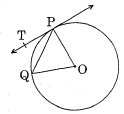
\includegraphics[width = 5cm,height = 5cm,center]{3.png}
\begin{enumerate}
    \item 55\degree
    \item 70\degree
    \item 45\degree
    \item 35\degree
\end{enumerate}
%\end{centering}
% \item In figure 1,O is the center of a circle,PQ is a chord and PT is the tangent at P.If $\angle POQ$ =$70\degree$ then $\angle TPQ $is equal to
% 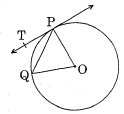
\includegraphics[width = \columnwidth]{3.png}
% \begin{enumerate}
%     \item 55\degree
%     \item 70\degree
%     \item 45\degree
%     \item 35\degree
% \end{enumerate}
%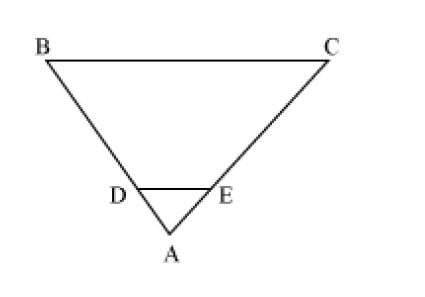
\includegraphics[width = \columnwidth]{2.png}
%If the sum of the first q terms of an arithmetic progression is $2q+3q^2$.What is the common difference?
%Find the value of m for which the pair of linear equations 2x + 3y – 7 = 0 and (m – 1) x + (m + 1) y = (3m – 1) has infinitely many solutions.\\
%\newcounter{rowno}
%\setcounter{rowno}{0}
%\begin{table}[!h]
%\centering
%\begin{tabular}{>{\stepcounter{rowno}\therowno.}cl}
%\multicolumn{1}{r}{No.} & text & abcd\\\hline
% & first  \\
% & second \\
% & third  \\
% & fourth 
%\end{tabular}
%\input{./line/tables/3d_ncert.tex}
%\caption{}
%\label{table:3d}
%\end{table}
\item In figure 2,AB and AC are the tangents to the circle with the center O such that $\angle BAC$ =$40\degree$.Then $\angle BOC $is equal to
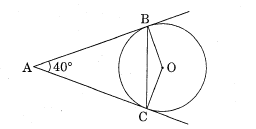
\includegraphics[width=\columnwidth]{4.png}
\begin{enumerate}
    \item 40\degree
    \item 50\degree
    \item 140\degree
    \item 150\degree
\end{enumerate}
%In Figure 1, CP and CQ are tangents from an external point C to a circle with centre O. AB are another tangent which touches the circle at R. If CP = 11 cm and BR = 4 cm, find the length of BC
%\begin{\centering}
%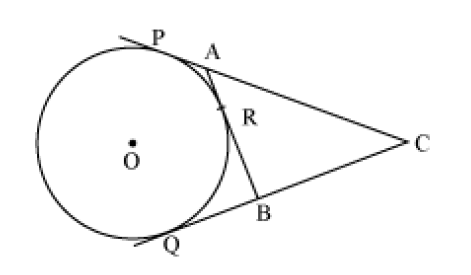
\includegraphics[width = \columnwidth]{1.png}
%\caption{}
%\label{fig:Line between A and B}
% \end{figure}
% \end{\centering}
%Solve the following pair of linear equations for x and y \\
%$\frac{b}{a}\vec{x}+\frac{a}{y}=a^2+b$\\
%$x+y = 2ab$\\



% then find the value of $p$.
\item The perimeter (in cm )of a square circumscribing a circle of radius a cm is
\begin{enumerate}
    \item 8a
    \item 4a
    \item 2a
    \item 16a
\end{enumerate}
%In Figure 2, $DE\parallel BC $in triangle  ABC such that BC = 8 cm, AB = 6 cm and DA = 1.5 cm. Find DE.

%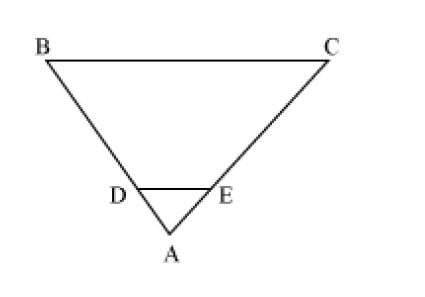
\includegraphics[width = \columnwidth]{2.png}

%If P($\frac{a}{2}$,4)is the midpoint of the line joining A (-6,5) and B (-2,3). Find a.\\
%\begin{enumerate}[itemsep=2pt]
%\begin{multicols}
%\item
$
%\myvec{2 & 3 & 4}\vec{x}=12
$
%\item
$
%\myvec{3 & 4 & -6}\vec{x}=0
$
%\item
$
%\myvec{1 & 1 & 1}\vec{x}=1
$
%\item
$
%\myvec{0 & 5 &0}\vec{x}=-8
$
%\end{multicols}
%\end{enumerate}
\item The radius(in cm) of the largest right circular cone that can be cut out from a cube of 4.2cm is
\begin{enumerate}
    \item 4.2
    \item 2.2
    \item 8.4
    \item 1.05
\end{enumerate}
%Find the value of y for which distance between points A (3,-1) and (11,y) is 10 units\\

\item A tower stands vertically on the ground. From a point on the ground which is 25 m away from the foot of the tower, the angle of elevation of the top of the tower is found to be 45°. Then the height (in meters) of the tower is
\begin{enumerate}
    \item 25$\sqrt{2}$\\
    \item 25$\sqrt{3}$ \\
    \item 25 \\
    \item 12.5
\end{enumerate}
%Find the value of x for which the distance between the points P(x,4) and Q (9,10) is 10 units\\
\item If P($\frac{a}{2},4)$ is the mid point of the line joining the points A(-6,5) and B(-2,3) then the value of a is
\begin{enumerate}
    \item -8
    \item 3
    \item -4
    \item 4
\end{enumerate}
%In a triangle ABC,right angled at C,AC=6cm and AB =12cm Find$ \angle A$
%8.	Find the value of k if the points P (5,4), Q (7, K) and R (9,-2) are collinear\\ %$\myvec{\sqrt{a^2-b^2}0}$ and $\myvec{\qrt{a^2-b^2}0}$ to the line 
%
%\begin{align}
%\myvec{\frac{\cos\theta}{a} & \frac{\sin\theta}{b}}\vec{x} &= 1
%\end{align}
%
%is $b^2$.
%\item Show that the lines 
%\begin{align}
%\frac{x-a+d}{\alpha-\delta} = \frac{y-a}{\alpha} &= %\frac{z-a-d}{\alpha+\delta}, 
\\
%\frac{x-b+c}{\beta-\gamma} = \frac{y-b}{\beta} &= %\frac{z-b-c}{\beta+\gamma} 
%\end{align}
%are coplanar.
\item If A and B are the points (-6,7) and (-1,-5) respectively, then the distance 2AB is equal to
\begin{enumerate}
    \item 13
    \item 26
    \item 169
    \item 238
\end{enumerate}
%The slant height of the frustum of a cone is 5 cm. If the difference between the radii of its two circular
%ends is 4 cm, write the height of the frustum.
%Find the coordinates of the point which divide the line segment joining A(2,-3) and B(-4,-6) in to three equal parts \\

\item A card is drawn from the well shuffled deck of 52 playing cards.The probability that the card will not be an ace is
\begin{enumerate}
    \item $\frac{1}{13}$
    \item $\frac{1}{4}$
    \item $\frac{12}{13}$
    \item $\frac{3}{4}$
\end{enumerate}
%A die is thrown once. What is the probability of getting a number greater than 4?
%Show that the points(3,5),B(6,0) ,C(1,-3) and D(-2,2) are the vertices of square ABCD

\item Find the value of m so that the quadratic equation mx(x-7)+49=0 has two equal roots
%Find the value of k for which the following pair of linear equation have infinitely many solutions:2x + 3y = 7; (k – 1) x + (k + 2)y = 3k \\
\item 
%Find the value of m for which the pair of linear equations 2x+3y-7=0 and (m-1)x
%Find the value of m such that the quadratic equation mx(x-7)+49=0 has equal roots
\item Find how many two digit numbers are divisible by 6
%Find the roots of the quadratic equation\\
$x^2-3\sqrt{5}x+10=0$ \\

\item In Figure 3,a circle touches all the four sides of a quadrilateral ABCD whose sides are AB=6cm,BC=9cm and CD=8 cm.Find the length of side AD.
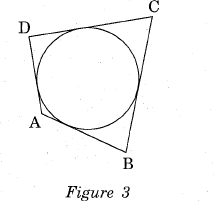
\includegraphics[width=\columnwidth,height=5cm,center]{5.png}
%Point P(x,4) lies on the line segment joining the points A(-5,8) and B(4,-10).Find the ratio the point P divides the line segment AB.Also find the value of x
\item Draw a line segment AB of length 7cm.Using a ruler and compassess,Find a point P on AB such that 
$\frac{AP}{AB}=\frac{3}{5}$
%Find he roots of the quadratic equation $x^2 +5x-(\(\alpha\) +1)(\(\alpha\) +6)= 0$,where \(\alpha\) is a constant 
\item Find the perimeter of shaded region in figure 4,if ABCD is a square of side 14cm and APB and CPD aere semicircles
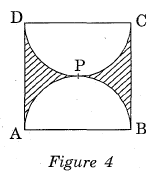
\includegraphics[width=5cm,height=5cm,center]{6.png}
%For what values of k does the quadratic equation\\
$(k-5)x^2+2(k-5)x+2=0 $ have equal roots
\item Two cubes each of volume 27 cm are joined end to end to form a solid. Find the surface area of the resulting cuboid.\\
%Find the roots of the following quadratic equation\\
%$\sqrt{3}x^2 - 2\sqrt{2}x-2\sqrt{3}=0$
OR\\
\item A cone of height 20 cm and radius of base 5 cm is made up of modelling clay. A child reshapes it in the form of a sphere. Find the diameter of the sphere.
%Find the are of the quadrilateral ABCD whose vertices are A(3,-1) ,B(6,0),C(14,0) and D(9,19)\\
\item Find the value of y for which the distance between the points A(3, -1) and B(11, y) is 10 units.
\item A ticket is drawn at random from a bag containing tickets numbered from 1 to 40. Find the probability that the selected ticket has a number which is a multiple of 5.

%Solve the following equation\\
%$\frac{1}{x+1}$+$\frac{2}{x+2}$=$\frac{5}{x+4}$, $x \neq -1,-2,-4$\
\item Find the roots of the following quadratic equation\\
$x^2-3\sqrt{5}x+10 =0$
%Find the root of the equation \\
%$\frac{1}{2x-3} + \frac{1}{x-5}=1$, $x \neq \frac{3}{2},5$.
\item Find an A.P. whose fourth term is 9 and the sum of its sixth term and thirteenth term is 40.
\item In Figure 5, a triangle PQR is drawn to circumscribe a circle of radius 6 cm such that the segments QT and TR into which QR is divided by the point of contact T, are of lengths 12 cm and 9 cm respectively. If the area of APQR = 189 cm”, then find the lengths of sides PQ and PR.
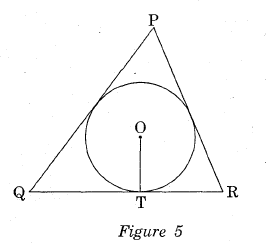
\includegraphics[width=5cm,height=5cm,center]{7.png}
\item Draw a pair of tangents to a circle of radius 3 cm, which are inclined to each other at an angle of 60\degree
\item Draw a right triangle in which the sides other than hypotenuse) are of lengths 4 cm and 3 cm. Then construct another triangle whose sides are $\frac{3}{5}$times the corresponding sides of the given triangle.\\
OR
\item A chord of a circle of radius 14 cm subtends an angle of 120° at the centre. Find the area of the corresponding minor segment of the circle.Use $\Pi$ =$\frac{22}{7}$ and$\sqrt{3}=1.73$\\
\item An open metal bucket is in the shape of a frustum of a cone of height 21 cm with radii of its lower and upper ends as 10 cm and 20 cm respectively. Find the cost of milk which can completely fill the bucket at Rs. 30 per litre
\item Point P(x, 4) lies on the line segment joining the points A(-5, 8) and B(4, - 10). Find the ratio in which point P divides the line segment AB. Also find the value of x.
\item Find the area of the quadrilateral ABCD, whose vertices are A(-3, -1), B(-2,-4), C(4, -1) and D(3, 4).\\
OR\\
\item Find the area of the quadrilateral ABCD, whose vertices are A(-3, -1), B(-2,-4), C(4, -1) and D(3, 4).
\item From the top of a vertical tower, the angles of depression of two cars, in the same straight line with the base of the tower, at an instant are found to be 45° and 60°. If the cars are 100 m apart and are on the same side of the tower, find the height of the tower. [Use $\sqrt{3} $= 1.73]
\item Two dice are rolled once. Find the probability of getting such numbers on the two dice, whose product is 12.\\
OR\\
\item A box contains 80 discs which are numbered from 1 to 80. If one disc is drawn at random from the box, find the probability that it bears a perfect square number.
\item Prove that the tangent at any point of a circle is perpendicular to the radius through the point of contact.
\item The first and the last terms of an A.P. are 8 and 350 respectively. If its common difference is 9, how many terms are there and what is their sum ?\\
OR\\
\item  How many multiples of 4 lie between 10 and 250 ? Also find their sum.
\item A train travels 180 km at a uniform speed. If the speed had been 9 km/hour more, it would have taken 1 hour less for the same journey. Find the speed of the train.\\
OR\\
\item Find the roots of the equation $\frac{1}{2x-3}$+$\frac{1}{x-5}$=1, x $\neq \frac{3}{2}$,5
\item In Figure 6, three circles each of radius 3-5 cm are drawn in such a way that each of them touches the other two. Find the area enclosed between these three circles (shaded region). Use $\Pi$ =$\frac{22}{7}$
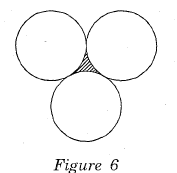
\includegraphics[width=5cm,height=5cm,center]{8.png}
\item Water is flowing at the rate of 15 km/hour through a pipe of diameter 14 cm into a cuboidal pond which is 50 m long and 44 m wide. In what time will the level of water in the pond rise by 21 cm ?
\item The angle of elevation of the top of a vertical tower from a point on the ground is 60°. From another point 10 m vertically above the first, its angle of elevation is 30°. Find the height of the tower.
\end{enumerate}
\end{document}\documentclass{article}
\usepackage[utf8]{inputenc}

\title{CBSE 2011 Class 10}

\begin{document}

\maketitle

\section{Introduction}

\end{document}
